\section{Khẩn cấp có cấu trúc, phân cụm và xếp hạng}\label{sec:02-data-methods-methods}
\subsection{Mô hình khẩn cấp Logistic Regression}\label{sec:02-urgency-lr}
Với vector cờ $\symbf{x}\in\{0,1\}^{5}$ của bảng 32 trạng thái (Mục~\ref{sec:02-data-methods-data}), mô hình v5 có dạng
\begin{equation}
 E_i^{\mathrm{LR}}=\operatorname{sigmoid}\!\left(\xi_0+\sum_{j=1}^{5}\xi_jx_j\right),
 \qquad \operatorname{sigmoid}(z)=\frac{1}{1+e^{-z}}.
 \label{eq:urgency-lr}
\end{equation}
JSON lưu $\xi_0=-1{,}0580446217$ và cả năm hệ số $\xi_j=1{,}1087792041$. Threshold kỹ thuật là 0,5 và \texttt{class\_weight=balanced}. Hệ số bằng nhau khiến đầu ra chỉ phụ thuộc số cờ được chọn trong không gian rút gọn. Đây không phải bằng chứng rằng năm dấu hiệu có trọng lượng y khoa như nhau; cấu trúc này phản ánh bảng huấn luyện đối xứng và nhãn OR của nhóm.

Trên toàn bộ 32 trạng thái, nhãn ở threshold 0,5 khớp quy tắc OR. Khi không có cờ, điểm bằng khoảng 0,2577; với một cờ, điểm nhỏ nhất của trạng thái dương khoảng 0,5127. Quy tắc OR trực tiếp là baseline chính xác cho định nghĩa nhãn này. Độ khớp toàn bảng và sanity test không chứng minh Logistic Regression tốt hơn quy tắc hoặc có hiệu quả lâm sàng.

Trong ứng dụng, điểm được tính từ các lựa chọn có cấu trúc và lưu ở trường \texttt{E\_i}. Mã backend hiện tại chưa dùng trường này khi chuyển sang \texttt{ReportV2}: adapter đọc \texttt{urgency} nếu có, nếu không thì dùng từ khóa mô tả. Vì vậy báo cáo phân biệt $E_i^{\mathrm{LR}}$ tại ứng dụng với $E_i$ đang thực sự đi vào phân cụm demo. Kết quả RQ2 và RQ3 không phải kết quả đánh giá mô hình LR.

\subsection{Biểu diễn báo cáo và điều kiện tiếp nhận}
Bản thảo nghiên cứu định nghĩa
\begin{equation}
 r_i=(L_i,T_i,F_i,E_i,N_i,V_i,Q_i),
 \label{eq:report-tuple}
\end{equation}
trong đó $L_i$ là vị trí GPS, $T_i$ là thời gian báo cáo quan sát, $F_i,E_i\in[0,1]$ là bằng chứng ngập và khẩn cấp, $N_i\geq0$ là số người được khai báo, $V_i\geq0$ là bằng chứng yếu thế và $Q_i$ là heuristic confidence/provenance. Ảnh hiện diện, loại nguồn và các cờ thiếu còn được dùng để xây fingerprint và confidence, nhưng không phải nhãn sự kiện.

Điều kiện vào đồ thị là $a_i=\mathbf{1}\{L_i,T_i\text{ được quan sát}\}$. Nếu $a_i=0$, báo cáo chuyển tới hàng xem xét. Việc chuyển hàng này giữ khả năng xử lý của con người thay vì tạo cạnh bằng một khoảng cách không xác định. Artifact RQ1 hiện tại có đầy đủ vị trí, thời gian và hai trường ngữ cảnh; nhánh thiếu dữ liệu là thiết kế và kiểm tra đơn vị, chưa có thực nghiệm thiếu dữ liệu trên chính bộ benchmark đó.

\subsection{Confidence từ dữ liệu quan sát}
Confidence dùng cho xếp hạng được tính bởi
\begin{equation}
 Q_i=\operatorname{sigmoid}\!\left(-0{,}2+1{,}4\,\mathbf{1}\{\text{có ảnh}_i\}
               +0{,}9\log(1+n_i^{\mathrm{corrob}})\right).
 \label{eq:confidence-report}
\end{equation}
$n_i^{\mathrm{corrob}}$ là số payload quan sát khác nhau củng cố lân cận, đếm theo định danh nội dung. Bản sao nguyên vẹn cùng payload không tự tạo thêm củng cố. Tuy nhiên, nhiều payload khác nhau được phối hợp có thể làm tăng confidence; cơ chế không chứng minh nguồn tin thật hoặc nguồn độc lập. Cách gom bản sao thành họ bằng chứng được định nghĩa ở Mục~\ref{sec:02-evidence-family}.

Confidence softmax của ảnh (Công thức~\ref{eq:softmax}), confidence/provenance trong payload và $Q_i$ có vai trò khác nhau. Trong adapter, confidence ảnh có thể được lưu làm provenance/fingerprint; điểm xếp hạng vẫn tính lại $Q_i$ theo Công thức~\ref{eq:confidence-report}. Nhầm hai loại confidence sẽ làm báo cáo giải thích sai nguyên nhân thay đổi ưu tiên.

\subsection{Độ tương đồng có xử lý thiếu ngữ cảnh}
Gọi $I_F(i,j)$ và $I_E(i,j)$ bằng một khi cả hai báo cáo có trường tương ứng, và $m_{ij}=I_F+I_E$. Độ tương đồng ngữ cảnh là
\begin{equation}
 C_{ij}=\frac{m_{ij}}{2}\exp\!\left[-I_F\frac{|F_i-F_j|}{\tau_F}
                                  -I_E\frac{|E_i-E_j|}{\tau_E}\right],
 \qquad C_{ij}=0\text{ nếu }m_{ij}=0.
 \label{eq:context-report}
\end{equation}
Với hai trường, mức tối đa bằng một; chỉ một trường thì mức tối đa giảm còn một nửa. Cách này tránh xem ``cùng thiếu'' như đồng thuận hoàn toàn. $\tau_F,\tau_E>0$ điều khiển mức suy giảm theo chênh lệch ngữ cảnh.

Với khoảng cách Haversine $d_{ij}$ theo mét và chênh lệch thời gian $\Delta t_{ij}$ theo phút,
\begin{equation}
 G_{ij}=\exp[-d_{ij}^{2}/(2\sigma^2)],\qquad
 T_{ij}^{\mathrm{sim}}=\exp[-\Delta t_{ij}/\tau_t].
 \label{eq:geo-time}
\end{equation}
Ký hiệu $T_{ij}^{\mathrm{sim}}$ phân biệt độ tương đồng thời gian với timestamp $T_i$. Hai cách hợp thành là
\begin{align}
 w_{ij}^{\times}&=a_ia_jG_{ij}(\beta T_{ij}^{\mathrm{sim}}+\gamma C_{ij}),\label{eq:product-graph}\\
 w_{ij}^{+}&=a_ia_j(\alpha G_{ij}+\beta T_{ij}^{\mathrm{sim}}+\gamma C_{ij}).\label{eq:additive-graph}
\end{align}
Dạng tích dùng không gian như cổng: dù thời gian và ngữ cảnh phù hợp, cạnh vẫn giảm nếu hai báo cáo xa nhau. Dạng cộng cho phép mỗi thành phần đóng góp độc lập. Động cơ cổng tích có liên hệ với cấu trúc spatial--range của bộ lọc bilateral \citep{tomasi1998bilateral}; toàn bộ công thức và lựa chọn tham số ở đây là định nghĩa của nghiên cứu nhóm, không phải một công thức cứu hộ chuẩn.

\subsection{Làm thưa đồ thị và phát hiện cộng đồng}
Pipeline tính ma trận cặp đủ điều kiện, xác định ngưỡng $\theta$ bằng quantile $q$ trên trọng số khác không, bỏ cạnh có $w\leq\theta$, chọn top-$K$ láng giềng còn lại theo từng đầu mút, rồi đối xứng bằng hợp các cạnh có hướng. Louvain hoặc Leiden được chạy trên đồ thị cuối với resolution đã khóa.

Top-$K$ ở mỗi đầu mút không bảo đảm bậc vô hướng của nút tối đa bằng $K$: nếu nhiều nút khác cùng chọn một nút thì bậc của nó có thể lớn hơn $K$. Quantile cũng phụ thuộc toàn bộ ma trận trọng số, nên khi thêm bản sao, phân bố cạnh và tập cạnh cạnh tranh có thể đổi dù từng bản sao có cùng nội dung. Đây là lý do cần kiểm tra riêng tính ổn định của phân cụm dưới multiplicity.

Bảng~\ref{tab:cluster-params} ghi các tham số của cấu hình Product được chọn ở RQ1 và các hằng số của điểm ưu tiên. Cấu hình Additive chọn $\alpha=1$ và $q=0{,}95$ cùng các tham số còn lại hiệu chỉnh riêng. Hai cấu hình được hiệu chỉnh độc lập nên phép so sánh chính là giữa hai pipeline được chọn, không phải tác động nhân quả của chỉ riêng phép tích hay phép cộng.

\begin{table}[htbp]\centering\small
\caption{Tham số của cấu hình Product (RQ1) và điểm ưu tiên}\label{tab:cluster-params}
\begin{tabular}{P{.30\textwidth}P{.15\textwidth}P{.38\textwidth}}
\toprule Tham số & Ký hiệu & Giá trị \\\midrule
Thang khoảng cách của cổng & $\sigma$ & 700 m \\
Thang thời gian & $\tau_t$ & 60 phút \\
Thang chênh lệch ngập, khẩn cấp & $\tau_F,\tau_E$ & 0,25; 0,35 \\
Trọng số thời gian, ngữ cảnh & $\beta,\gamma$ & 0,5; 0,5 \\
Quantile ngưỡng cạnh & $q$ & 0,90 \\
Số láng giềng giữ lại & $K$ & 8 \\
Resolution của Louvain/Leiden & --- & 1,2 \\
Hệ số của $Q_i$ & --- & $-0{,}2$; $1{,}4$; $0{,}9$ (Công thức~\ref{eq:confidence-report}) \\
Trọng số điểm ưu tiên & $\omega_E,\omega_F,\omega_N$ & 0,34; 0,33; 0,33 \\
Hệ số cực đại, thang yếu thế & $\mu,\ s$ & 2; 10 \\
Mốc số người, trần yếu thế & $N_{\mathrm{ref}},\ V_{\mathrm{cap}}$ & 500; 50 \\
\bottomrule\end{tabular}
\end{table}

\begin{figure}[htbp]
\centering
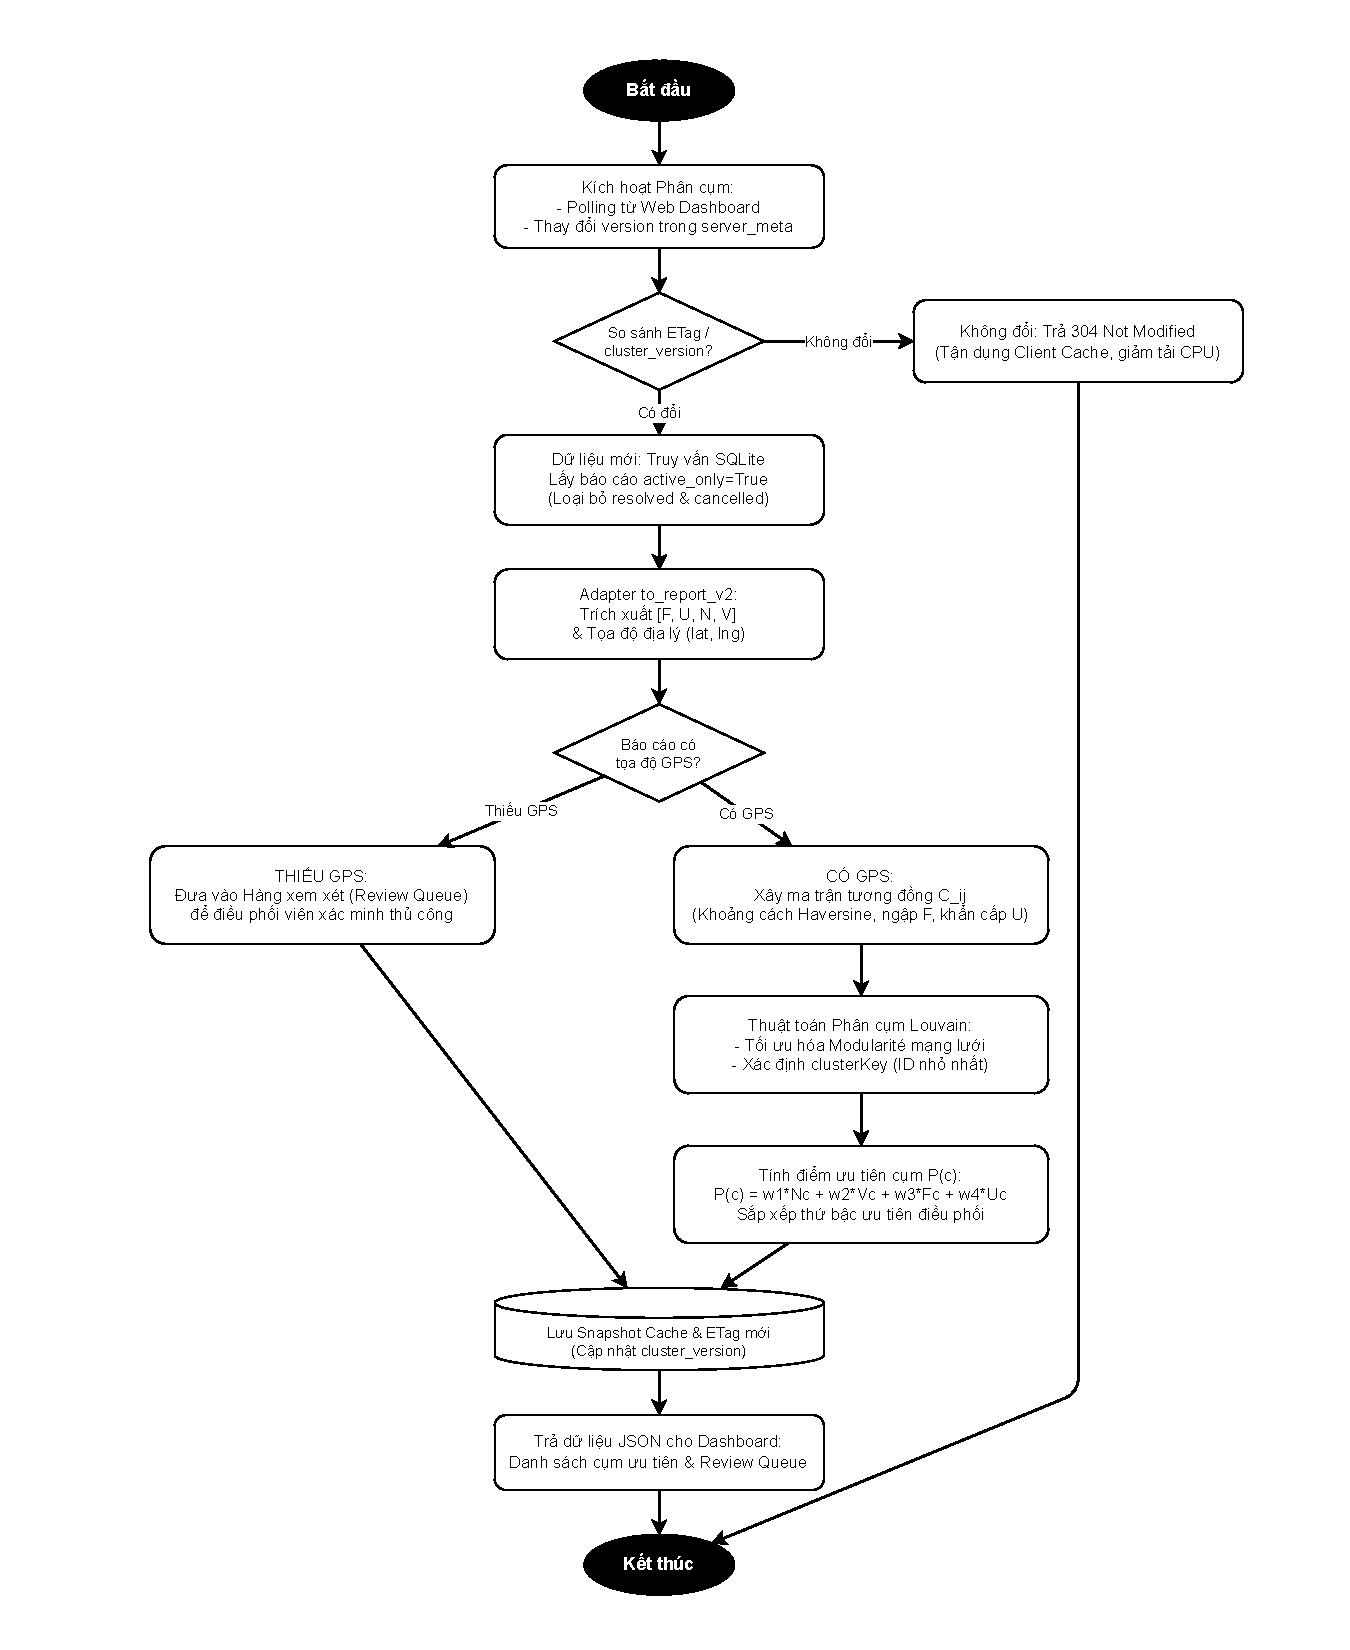
\includegraphics[width=.95\textwidth]{flow_06_clustering_priority.pdf}
\caption{Quy trình phân cụm đồ thị không gian Louvain và tính điểm ưu tiên cứu hộ $P(c)$}
\label{fig:flow-clustering-priority}
\end{figure}

\subsection{Chặn khoảng cách cạnh và giới hạn của bảo đảm}
Đặt $B=\beta+\gamma>0$. Vì $a_ia_j\leq1$ và $T_{ij}^{\mathrm{sim}},C_{ij}\leq1$,
\begin{equation}
 w_{ij}^{\times}\leq B\exp[-d_{ij}^2/(2\sigma^2)].
 \label{eq:edge-upper}
\end{equation}
Nếu cạnh được giữ với $0<\theta<B$, kết hợp $\theta<w_{ij}^{\times}$ và lấy log cho
\begin{equation}
 d_{ij}<r_{\theta}^{\times}=\sigma\sqrt{2\log(B/\theta)}.
 \label{eq:edge-radius}
\end{equation}
Khi $\theta\geq B$, tập giữ theo bất đẳng thức nghiêm là rỗng; khi $\theta\leq0$, ngưỡng này không cho chặn khoảng cách hữu hạn.

Chặn trên chỉ áp dụng từng cạnh. Một chuỗi nhiều cạnh ngắn vẫn có thể tạo thành phần rộng (Hình~\ref{fig:edge-chain}). Nếu thành phần không đơn có đường kính theo số bước $h$, bất đẳng thức tam giác cho đường kính địa lý $D<hr_{\theta}^{\times}$. Đây là chặn có điều kiện sau khi quan sát $h$, vì thuật toán không áp một chặn trước cho $h$.

Với dạng cộng và $\alpha>0$, chặn hữu hạn từ threshold chỉ có khi $B<\theta<B+\alpha$:
\begin{equation}
 d_{ij}<\sigma\sqrt{2\log\!\left(\frac{\alpha}{\theta-B}\right)}.
 \label{eq:additive-bound}
\end{equation}
Các thuộc tính này làm rõ cấu trúc đồ thị, nhưng không chứng minh Product có ARI cao hơn hoặc lịch điều phối tốt hơn. Kết quả thực nghiệm được đánh giá độc lập với bảo đảm toán học.

\begin{figure}[htbp]\centering
\begin{tikzpicture}[>=Stealth,font=\small,
 pt/.style={circle,draw,minimum size=9mm}]
\node[pt] (a) at (0,0) {$r_1$};
\node[pt] (b) at (3,0) {$r_2$};
\node[pt] (c) at (6,0) {$r_3$};
\node[pt] (d) at (9,0) {$r_4$};
\draw[thick] (a)--node[above]{$d<r_\theta^\times$}(b);
\draw[thick] (b)--node[above]{$d<r_\theta^\times$}(c);
\draw[thick] (c)--node[above]{$d<r_\theta^\times$}(d);
\draw[<->] (0,-1)--node[below,align=center]{Hai đầu chuỗi có thể xa hơn $r_\theta^\times$\\dù mọi cạnh đều thỏa chặn}(9,-1);
\end{tikzpicture}
\caption{Ví dụ khái niệm: chặn chiều dài cạnh không chặn trực tiếp đường kính cộng đồng}
\label{fig:edge-chain}
\end{figure}

\subsection{Chi phí tạo đồ thị và tác động của multiplicity}
Tính tương đồng đầy đủ cho $n$ báo cáo cần xét $n(n-1)/2$ cặp. Khi cài bằng ma trận dense, chi phí lưu trữ là $O(n^2)$; bước làm thưa chỉ giảm số cạnh ở đồ thị cuối, chưa loại chi phí tạo ma trận ban đầu. Hợp của các lựa chọn top-$K$ có tối đa $nK$ cạnh vô hướng trước khi bỏ cạnh trùng, nhưng bậc của từng nút vẫn có thể vượt $K$ như đã giải thích. Với bộ benchmark vài trăm báo cáo mỗi run, thiết kế này phù hợp cho khảo sát lõi; khả năng vận hành ở quy mô lớn cần phép đo tải riêng.

Nếu sao chép làm kích thước đầu vào tăng khoảng $m$ lần, số cặp trước làm thưa tăng xấp xỉ $m^2$ lần. Đồng thời, nhiều cạnh bản sao xuất hiện trong phân bố dùng chọn quantile và trong cạnh tranh top-$K$. Đây là cơ chế có thể giải thích vì sao bất biến điểm khi grouping cố định không kéo theo bất biến phân cụm. Kết quả stress chỉ cho thấy hiện tượng, chưa cô lập tỷ lệ đóng góp của threshold, top-$K$ hay bước tối ưu cộng đồng.

Khử transport copy trước khi tạo đồ thị là một hướng giảm số nút lặp, nhưng cần giữ lineage để evaluator vẫn đánh giá trên đơn vị báo cáo gốc theo protocol. Nếu tự bỏ các hàng trùng rồi đổi mẫu số ARI, phép so sánh trước và sau sẽ đổi cả thuật toán lẫn bài toán đánh giá. Tương tự, chỉ giữ gần trùng bằng envelope có thể gộp quan sát độc lập; cần kiểm tra cả sai gộp và sai tách khi thử hướng này.

\subsection{Họ bằng chứng và tổng hợp có chặn}\label{sec:02-evidence-family}
Trong cụm dự đoán thứ $k$, bản sao exact được nhận diện bằng fingerprint chuẩn tắc; bản gần trùng được liên kết bằng thành phần liên thông trong envelope quan sát. Mỗi nhóm bản sao như vậy là một \emph{họ bằng chứng}. Phương pháp gần trùng có tính bắc cầu, không phải complete linkage. Ký hiệu $\mathcal F_k$ là tập họ bằng chứng trong cụm $k$. Đặt $\widetilde N_i=\min(N_i,N_{\mathrm{ref}})$ và $\widetilde V_i=\min(V_i,V_{\mathrm{cap}})$.
\begin{align}
 \bar E_k&=\frac{\sum_{g\in\mathcal F_k}\max_{i\in g}Q_iE_i}
                    {\max(1,\sum_{g\in\mathcal F_k}\max_{i\in g}Q_i)},\label{eq:aggregate-e}\\
 \bar F_k&=\max_{g\in\mathcal F_k}\max_{i\in g}Q_iF_i,\label{eq:aggregate-f}\\
 \bar N_k&=\min\!\left(1,\frac{\log(1+\max_{g\in\mathcal F_k}\max_{i\in g}Q_i\widetilde N_i)}{\log(1+N_{\mathrm{ref}})}\right),\label{eq:aggregate-n}\\
 \bar V_k&=\max_{g\in\mathcal F_k}\max_{i\in g}Q_i\widetilde V_i.\label{eq:aggregate-v}
\end{align}
Cực đại theo họ hạn chế việc coi nhiều bản tin chồng lặp là những nhóm người rời nhau. Log nén miền số người, clipping giới hạn một khai báo và confidence điều tiết đóng góp. Tuy nhiên, cực đại có thể bị chi phối bởi khai báo cao không đúng; đây là một giả định phương pháp cần kiểm tra.

Điểm ưu tiên là
\begin{equation}
 P_k=\left[1+(\mu-1)\tanh(\bar V_k/s)\right]
       (\omega_E\bar E_k+\omega_F\bar F_k+\omega_N\bar N_k).
 \label{eq:priority-report}
\end{equation}
Nguồn Candidate 4.1 và lõi demo dùng các hằng số ở Bảng~\ref{tab:cluster-params}. Với trọng số không âm có tổng một, $\bar E_k,\bar F_k,\bar N_k\in[0,1]$ và $\bar V_k\geq0$, suy ra $0\leq P_k\leq\mu$. Các hằng số chưa được xem là trọng số chính sách đã có xác nhận chuyên gia.

Nếu họ bằng chứng và các đầu vào đã khóa, thêm bản sao exact không đổi cực đại trong họ, không tạo payload củng cố mới và không đổi $Q_i$. Vì vậy các đại lượng tổng hợp và $P_k$ không đổi. Điều kiện này cần được giữ trong phát biểu: thay đổi phân hoạch hoặc họ bằng chứng có thể phá vỡ tính bất biến của toàn pipeline.
